\begin{auf}
    852
\end{auf}
Eine dünne plankonvexe Linse aus Glas ($n=1.5$) liegt mit der sphärisch gekrümmten Fläche auf einer ebenen Glasplatte. Die Linse wird senkrecht von oben mit monochromatischem Licht der Wellenlänge $\lambda$ beleuchtet. Mit einem Messmikroskop wird der Radius des dunklen NEWTONschen Ringes 1. Ordnung zu $r_1=840mm$, der Radius 5. Ordnung zu $r_5=1180mm$ ausgemessen (Blickrichtung von oben).
\begin{enumerate}
    \item[a] An welchen	beiden Grenzflächen werden die interferierenden Strahlen reflektiert?
    \item[b] Wie groß ist $\lambda$, wenn der Krümmungsradius der Linse	$R=350mm$ beträgt?
    \item[c] Was beobachtet man im Zentrum, wenn die Linse exakt auf der Glasplatte aufliegt?
\end{enumerate}
\begin{figure}[h]
    \centering
    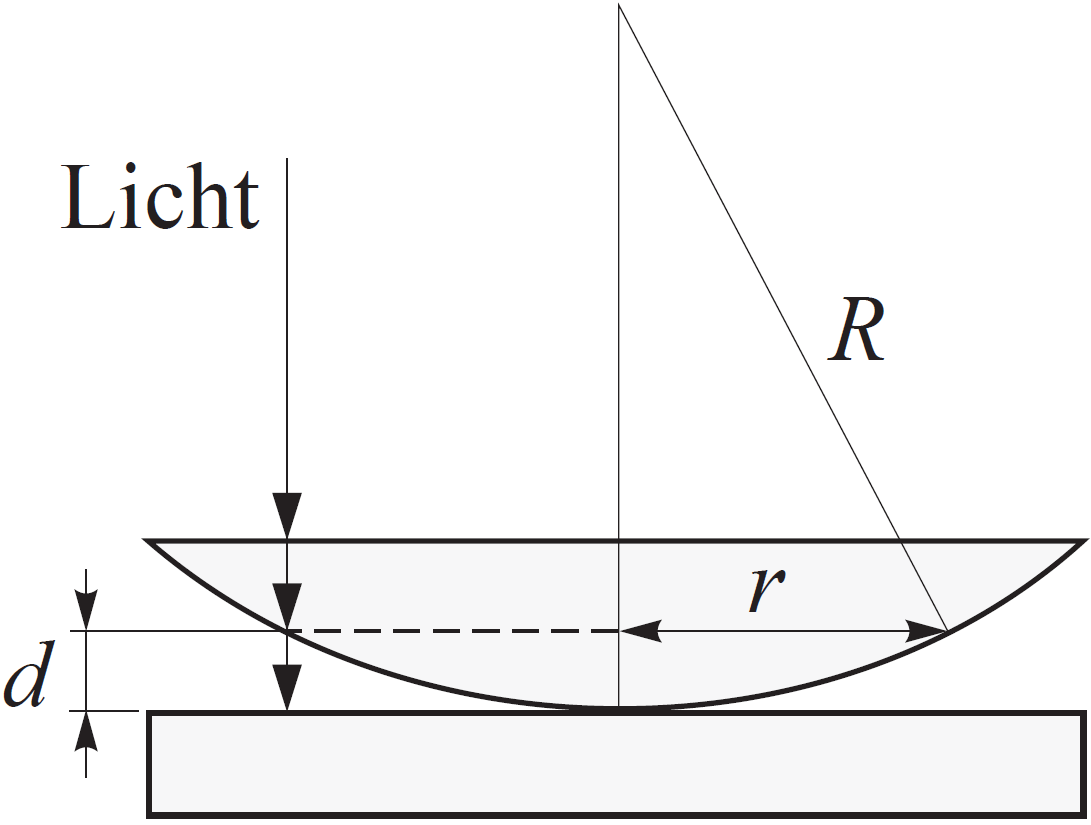
\includegraphics[height=5cm]{images/852_0.png}
    \caption{Versuchsaufbau Aufgabe 852}
\end{figure}